\documentclass[11pt, conference]{article}
\usepackage[left=4cm, right=4cm, top=3cm, bottom=3cm]{geometry}
\usepackage{graphicx}
\usepackage{cite}
\usepackage{algorithmic}
\usepackage{graphicx}
\usepackage{textcomp}
\usepackage{balance}
\usepackage{comment}
\usepackage{grffile}
\usepackage{subcaption}
\usepackage{lipsum}
\usepackage{float}

\newcommand{\vectorScheme}{\textit{Vector Scheme}}
\newcommand{\valueScheme}{\textit{Value Scheme}}
\newcommand{\distanceScheme}{\textit{Distance Scheme}}
\newcommand{\distanceLemma}{\textit{Distance Lemma}}
\newcommand{\sketchScheme}{\textit{Sketched Data Scheme}}
\newcommand{\fullSync}{\textit{Full Sync}}
\newcommand{\naiveScheme}{\textit{Naive Scheme}}
\newcommand{\oracleScheme}{\textit{Oracle Scheme}}
\newcommand{\falseAlarm}{\textit{false alarm}}
\newcommand{\falseAlarms}{\textit{false alarms}}
\newcommand{\coveringSpheres}{\textit{Covering Spheres}}
\newcommand{\convexDecomposition}{\textit{Convex Decomposition}}
\newcommand{\convexBound}{\textit{Convex Bound}}
\newcommand{\theCoordinator}{\textit{the coordinator}}
\newcommand{\Coordinator}{\textit{Coordinator}}
\newcommand{\TheCoordinator}{\textit{The coordinator}}
\newcommand{\safeZone}{\textit{safe zone}}

\begin{document}
	\begin{titlepage}
		\begin{center}
			\vspace*{1cm}
			\begin{Huge}
				Thesis Proposal \\
			\end{Huge}
			\vspace{1cm}
			\line(1,0){300} \\
			\vspace{0.2cm}
			\begin{Huge}
				Bandwidth Efficient Distributed Monitoring Schemes \\
			\end{Huge}
			\line(1,0){300} \\
			\vspace{1.5cm}
			\begin{Large}
				November 2018 \\
			\end{Large}
			\vspace{1.5cm}
			\begin{large}
				Written by Yuval Alfassi \\
				\textit{Computer Science Department} \\
				\textit{University of Haifa} \\
				yuvalalfassi@gmail.com \\
			\end{large}
			\vspace{2cm}
			\begin{large}
				Supervised by Prof. Daniel Keren \\
				\textit{Computer Science Department} \\
				\textit{University of Haifa} \\
				dkeren@cs.haifa.ac.il \\
			\end{large}
		\end{center}
	\end{titlepage}

\newgeometry{top=1.5in,bottom=1.5in,right=1in,left=1in}

\section*{Abstract}

Distributed monitoring is a problem that arises when trying to monitor properties of dynamic data which is spread distributively. Tracking the value of a function over dynamic data in a distributed setting is a challenging problem in numerous real-world modern applications. Several monitoring schemes were proposed as an approach to coping with this problem in order to reduce the amount of communication messages between servers.

Here, we'll propose several new distributed monitoring schemes which use much less communication bandwidth than existing methods. Whereas existing schemes send high dimensional vectors from server to server, we'll propose some innovative methods for reducing the dimensionality of the transmitted data even down to one single scalar. This will be done by exploiting some unique traits of convex functions.

\section{Introduction}

Monitoring a function over large amount of dynamically changed data in a distributed fashion is a common computer-science challenge. Whether it's monitoring features of distributed sensor networks \cite{burdakis2012detecting}, top-k monitoring \cite{babcock2003distributed}, monitoring distributed ratio queries \cite{gupta2013ratio} or tracking properties of large distributed dynamic graphs \cite{mcgregor2015densest}, innovative approaches had to be developed in order to deal with the difficulties of both the data being dynamic and distributed.

The need of minimizing both the bandwidth and the processing power is expressed in \cite{giatrakos2013network}; in the \textit{Big Data} era, where data is of very high dimensionality and changes rapidly, data transmition over a communication channel has to be planned cleverly. Transmition of high dimensional data is not only impractical, but also extremely time consuming; for instance, air pollution sensors which distributively have to determine the air pollution level may benefit from an economical communication approach \cite{cheng2004revised}.

\subsection{Problem Definition}

Commonly, distributed monitoring schemes are focused on determining whether a function over dynamic distributed data crosses a certain threshold. This is used as a component to the \textit{distributed function approximation problem} \cite{garofalakis2013sketch}, which $\varepsilon$-approximates the value of a function over time. The distributed model is described as follows:
\begin{enumerate}
\item There are $n$ data-servers, $server_1 ... server_n$
\item A central \textit{coordinator} exists, with whom the servers communicate over a communication channel.
\item $Server_i$ knows only its dynamic data -- the local vector, $v_i$.
\item The global data, represented by the \textit{global vector} $v$, is the average of the local vectors:
\begin{equation}
v = \frac{1}{n}\sum\limits_{i=1}^n {v_i}
\end{equation}
\item A function $f$ is monitored over the \textit{global vector} $v$ so it's $\varepsilon$-approximated with 100\% confidence: let the estimation be the dynamic value $\mu$ (without loss of generality, assume ${\mu \geq 0}$), then at all times: 
\begin{equation}
(1-\varepsilon )\mu \leq f(v) \leq (1+\varepsilon )\mu
\end{equation}
\end{enumerate}

The \textit{threshold monitoring problem} \cite{garofalakis2013sketch}  monitors whether the function's value crosses a certain threshold. The function approximation problem is commonly reduced to two simultaneous threshold monitoring problems: let ${T = (1+\varepsilon )\mu}$ be the upper-bound threshold's value, then, the upper-bound monitoring objective is to determine whether:
\begin{equation}
f(v) \leq T
\end{equation}

Likewise, the lower-bound function monitoring is done with the threshold ${(1-\varepsilon )\mu}$.

In turn, this threshold monitoring can be treated as a \textit{geometric monitoring problem} \cite{sharfman2007geometric}, where one tries to find a \safeZone \ of vectors ${\{v \ | \ f(v) \leq T\}}$, which is a convex, so every linear combination of vectors inside this \safeZone \ is also inside the \safeZone , see Fig. \ref{fig:ConvexSafeZoneSketch}. This geometric safe zone approach is the fundamental idea behind distributed monitoring techniques.

\begin{figure}[h]
\begin{center}
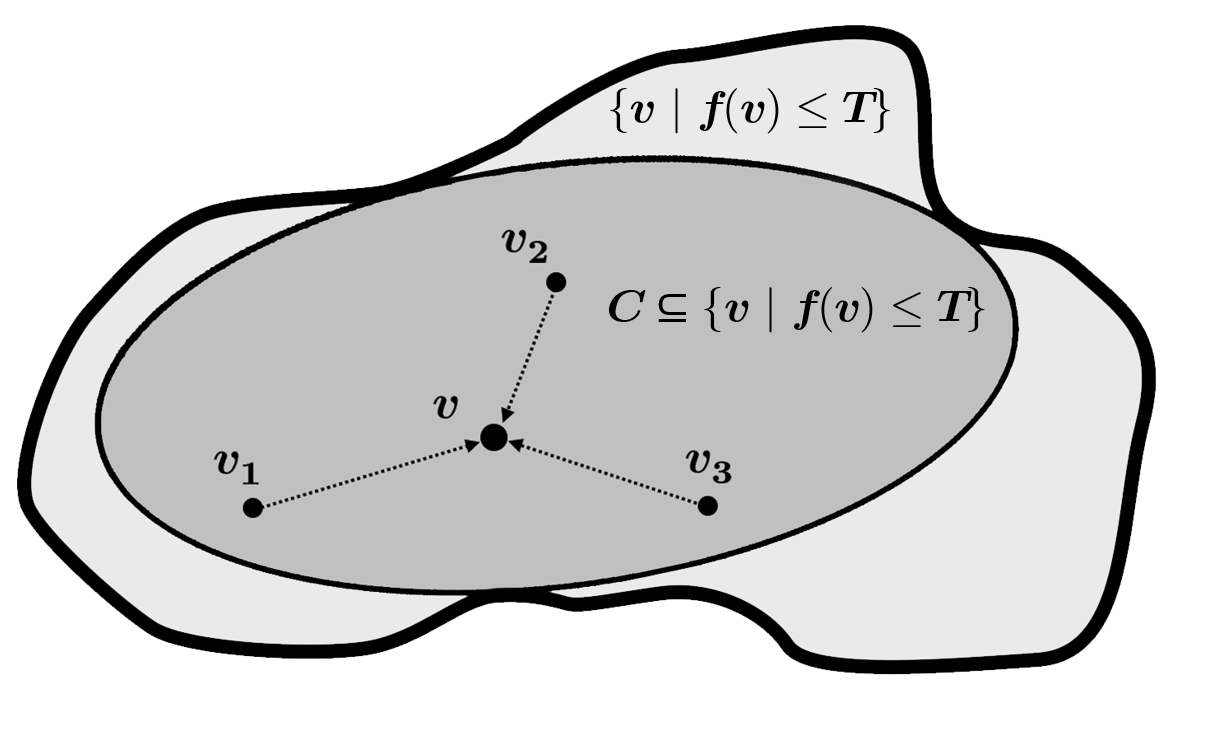
\includegraphics[width=0.6\linewidth]{Pics/PNGs/ConvexSafeZone.png}
\end{center}
\caption{Convex Safe Zone}
\label{fig:ConvexSafeZoneSketch}
\medskip
\small
\begin{center}
$C$ is a convex subspace of ${\{v \ | \ f(v) \leq T\}}$ so since ${v_1,v_2,v_3 \in C}$, so does the average vector $v \in C$.
\end{center}
\end{figure}

\section{Previous Work}

\subsection{Linear Functions}

Since linear functions are additive and homogeneous, the basic algorithm for distributively monitoring their value is fairly easy. Since ${f(v) = \frac{1}{n}\sum f(v_i)}$, tracking the value of the global $f(v)$ isn't quite complicated. A work about linear functions such as the distributed count problem was done at \cite{keralapura2006communication}. However, things get more sophisticated when dealing with non-linear functions.

\subsection{The Covering Spheres Method}

The first approach which exploited some geometric traits of the ditributed monitoring problem is the \coveringSpheres \ method \cite{sharfman2007geometric}.

This method artificially creates a convex safe zone subspace (as shown in Fig. \ref{fig:ConvexSafeZoneSketch}) where change vectors could be at without a need for communication.

This method seemed very effective theoratically, though it proved to be impractical. The \coveringSpheres \ method demands performing lots of time consuming heavy mathematical operations, so it isn't scalable computation-wise.

Furthermore, the violation resolution phase demands transmitting high dimensional vectors, which makes the communication bandwidth quite too high.

\subsection{The Convex Decomposition Method}

Another distributed monitoring scheme previously developed is the \convexDecomposition \ method \cite{lazerson2015monitoring}. This method composes a convex safe zone by decomposing the space ${\{v \ | \ f(v) \leq T\}}$ into convex subspaces and geometrically monitoring whether the average global vector is in their intersection.

Unfortunately, this method suffers from similar issues as the \coveringSpheres \ method, and cannot be applied on some basic functions, thus isn't feasable \cite{lazerson2018lightweight}

\subsection{The Convex Bound Method}

The \coveringSpheres \ method and the \convexDecomposition \ method turned out to be impractical albeit their mathematical purity. In need of more computationally lightweight and consistent monitoring approach, the \convexBound \ method was proposed \cite{lazerson2018lightweight}.

The \convexBound \ method simply bounds the monitored function by a convex function, so the convex bound serves as the convex safe zone: when monitoring $f(v) \leq T$, an upper bound convex $c$ has to be found so for all $v$, $f(v) \leq  c(v)$.

And the new monitoring objective becomes:
\begin{equation}
\label{monitoringConstraint}
c(v) \leq T
\end{equation}

The same goes for lower bound threshold monitoring -- It's done by bounding $f$ from below by a concave function.

\begin{figure}[t]
\begin{center}
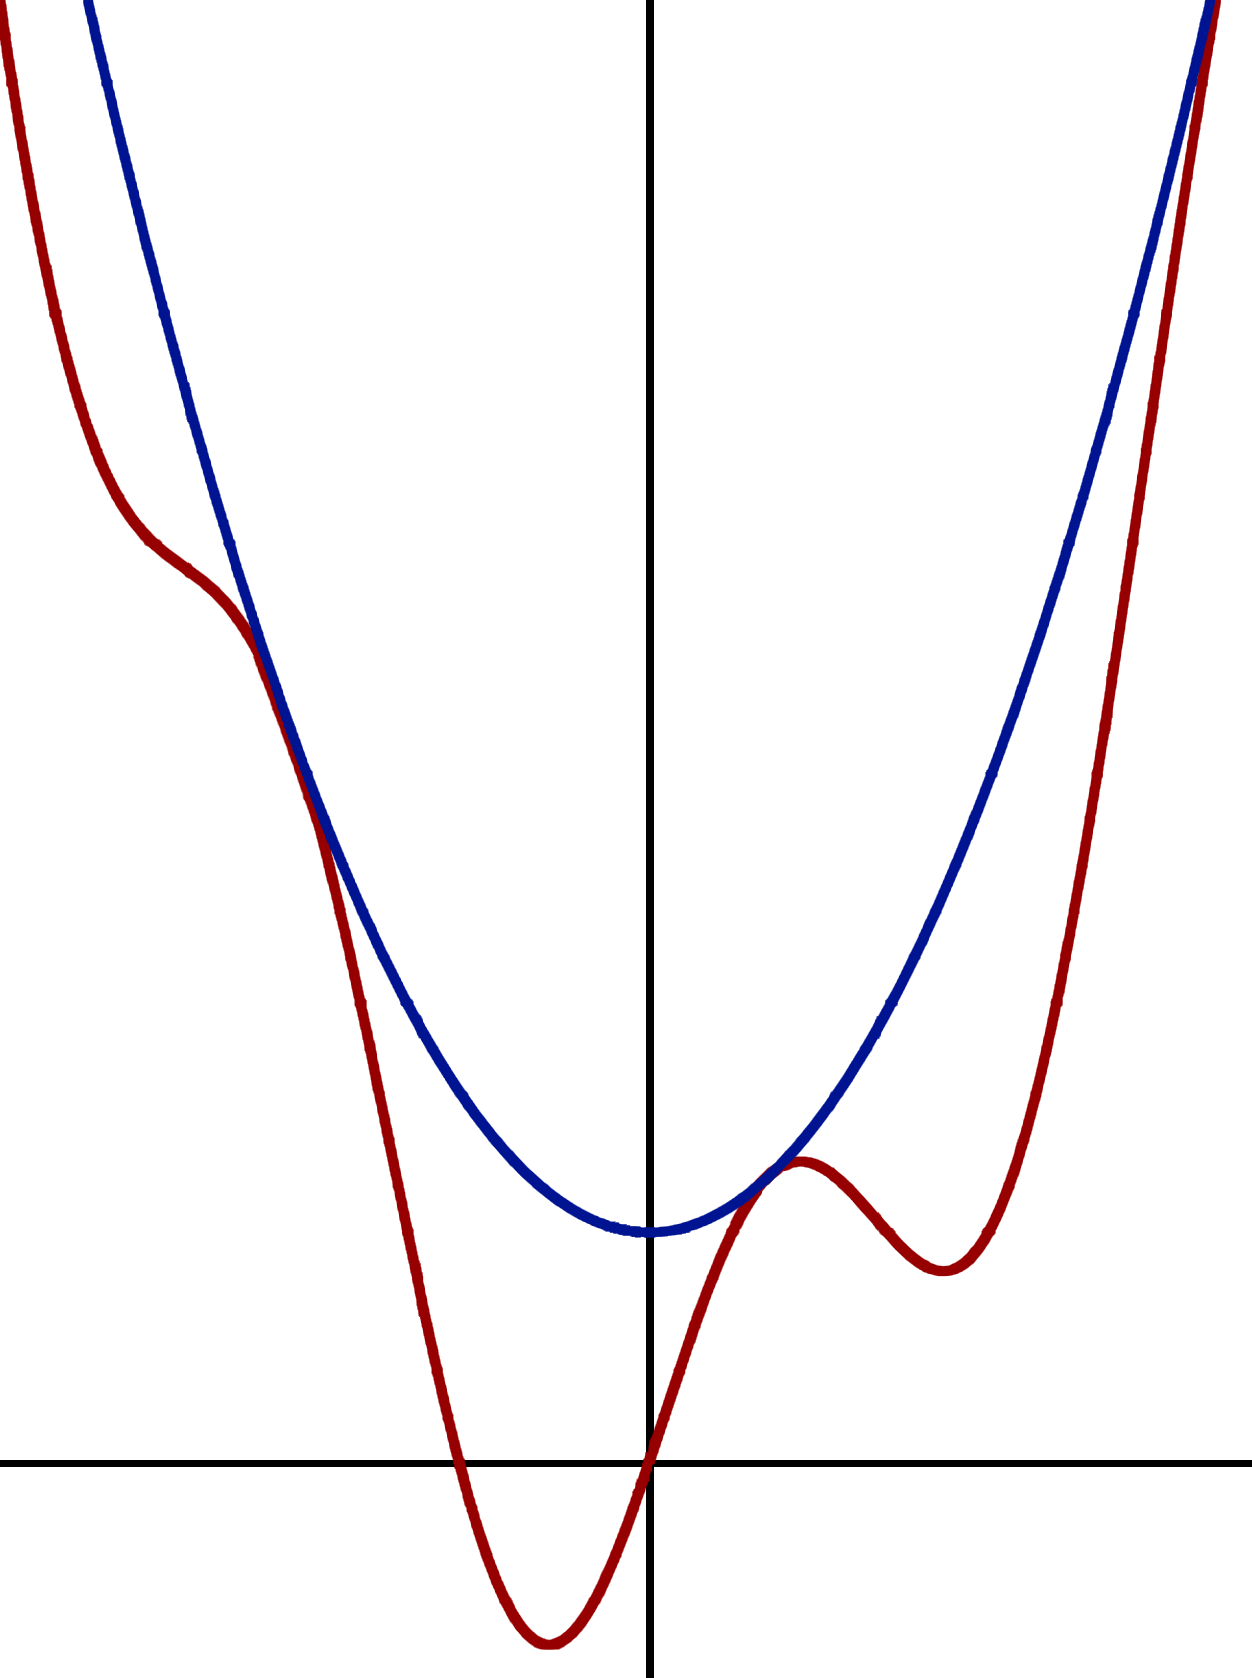
\includegraphics[width=0.3\linewidth]{Pics/PNGs/ConvexBound.png}
\end{center}
\caption{$x^2+10$ is an upper convex bound of $x^2+10sin(x)$}
\end{figure}

Accordingly, the distributed function monitoring is done on the convex bound functions, which is far simpler due to the convexity property.

\section{Research Objectives}

\begin{enumerate}
\item Introducing multiple innovative distributed monitoring schemes which avoid sending big dimensional data unless its crucially needed.

\item Proving the \distanceLemma , a lemma used as a basis of an efficient distributed monitoring scheme we'll develop. The \distanceLemma \ states that given a convex body and several points, if the sum of distances to the convex border from the points inside the convex body is greater than the sum of distances to the border from the points on the outside, then the average of the points is inside the convex body.

\item Incorporating data-sketches into distributed monitoring schemes without damaging the 0\% false-negative necessity of the distributed monitoring problem.

\item Conducting several experiments, laying out comparisons of multiple attributes of distributed monitoring schemes on real-world data, focusing on the bandwidth consumption.
\end{enumerate}

\bibliographystyle{ieeetran}
\bibliography{References}
	
\end{document}